\chapter{Composite ALP Matching}\label{ALP_match}

%%%%%%%%%%%%%%%%%%%%
\section{UV Lagrangian \label{sec:model}}
%%%%%%%%%%%%%%%%%%%%

As a case study, we consider a particular BSM model which gives rise to an effective axion model with flavor off-diagonal lepton couplings: the composite dark matter and composite neutrino model of Ref.~\cite{Davoudiasl:2017zws}. Ref.~\cite{Davoudiasl:2017zws} provides a UV realization of their model by introducing two vector-like fermions with charge $F$ and $F'$ and $(3, 2, -1/2, +)$ and $(3, 2, -1/2, -)$ under $SU(3)_D \times SU(2)_L\times U(1)_Y \times {\Bbb Z}_2$, along with a generational triplet of scalars $S_a$ with $a = e,\mu,\tau$ and quantum numbers $(3, 1, 0, +)$. The resulting UV Lagrangian is\footnote{The $S$-$\psi_i$-$\psi_j$ interaction requires that the $S$ doesn't couple to the usual current $\bar{\psi}_i\psi_j$, but instead to $\bar{\psi}_i^c \psi_j$. This is because the decomposition $3\times\bar{3}\times 3 = 3\oplus 3\oplus 6\oplus 15$ does not contain a singlet, whereas $3\times 3 \times 3 = 1 \oplus 8 \oplus 8 \oplus 10$ does. The color contractions for the $S$ and $\psi_i$ are suppressed; explicitly, $S_a \bar{\psi}_i^c \psi_j \sim \epsilon_{\alpha\beta\gamma}(S_a)_\alpha (\bar{\psi}^c_i)_\beta (\psi_j)_\gamma$. 
}
\begin{align}
    {\cal L}_{\rm UV} &= \lambda_1 \tilde{H}^*\bar{F}\psi_1 + \lambda_2\tilde{H}^*\bar{F}\psi_2 + \lambda_3 \tilde{H}^*\bar{F}'\psi_3 \nonumber \\
    &+ \lambda_a' S_a \bar{F}L_a + \sum_{i,j=1}^{3}\left.S_a\bar{\psi}_i^c\left[g_{aS}^{ij}+ig_{aPS}^{ij}\gamma^5\right]\psi_j\right|_{{\Bbb Z}_2 = +} \nonumber \\
    &+ \mu_S S_e S_\mu S_\tau + {\rm H.c.}\label{eq:UV_lag} 
\end{align}


The scalar $S$ and vector-like fermions $F$ are heavy states, which when integrated out leave an effective Lagrangian containing the ``dark quark" fields $\psi_i$ and the Standard Model Higgs field $H$ and left-handed lepton doublets $L_a$.  The dark quark fields carry a $\mathbb{Z}_2$ discrete symmetry under which only $\psi_3$ is odd; the other fields carry appropriate $\mathbb{Z}_2$ charges so that the Lagrangian is invariant. 

The dark quarks are charged under a confining $SU(3)_D$ gauge interaction, so that below the dark confinement scale $\Lambda_D$ the appropriate degrees of freedom are meson-like and baryon-like states formed from the $\psi_i$.  The low-lying spectrum of composite states in this theory include $N \sim (\psi_i^3)$ ``dark neutrons'', which play a role in neutrino mass generation, and $\kappa \sim (\bar{\psi}_i \psi_3)$ ``dark kaons,'' the lightest of which is stable and provides a dark matter candidate.  The four remaining light meson states,   a ``dark pion'' triplet $\Pi \sim (\bar{\psi}_1 \psi_2)$ and an equivalent of the $\eta$ meson, are unstable and can be identified as axion-like particles at low energies.

To match on to a low-energy effective Lagrangian, the unstable dark meson states should be identified as four different ALP states.  In practice, following the parameters of the UV completion, we will assume that these states are degenerate and match on to the simplifed Lagrangian  Eqs.~\ref{eq:dark_pion_int}-\ref{eq:dark_pion_Higgs} by introducing counting factors to treat them as a single $a$ state.  Exploration of the dynamics of composite ALP states where mass splittings are important would be interesting to consider in future work.

\section{Higgs couplings}

We begin by consideration of the Higgs-dark pion couplings to determine $C_{ah}$ and $C_{ah}'$ in the ALP Lagrangian.  For pions in the Standard Model, both couplings arise; however, the derivative $C_{ah}$ coupling arises due to matching from the coupling of the Higgs to the gluonic $G \tilde{G}$ operator, which in turn is induced by integrating the heavy quarks $c,b,t$ out of the theory.  In the present model, there are no such heavy dark fermions, so that the Higgs coupling to axions is entirely due to matching on to the same operator $h \bar{\psi}_i \psi_i$ which is responsible for generation of dark fermion mass.  This leads to generation of only the $C_{ah}'$ operator when matching at leading order.  We have
%
\begin{equation}
\mathcal{L}_{\Pi h} = \sum_{\Pi} \frac{1}{2v} M_\Pi^2 \Pi^2 h =  \sum_{\Pi} \frac{C'_{\Pi h}}{\Lambda^2} v M_\Pi^2 \Pi^2 h
\end{equation}
%
where the sum is over the four light meson states, and we are defining the effective coupling
%
\begin{equation}
\frac{C'_{\Pi h}}{\Lambda^2} \equiv \frac{1}{2v^2}.
\end{equation}
%
This is not quite the same as $C'_{ah}$, due to the fact that there are multiple $\Pi$ states but only a single $a$ in the ALP EFT Lagrangian (\ref{eq:ALP_EFT}).  This leads to an enhancement of $\Gamma(h \rightarrow \Pi \Pi)$ by a factor of 4 relative to the magnitude of $\Gamma(h \rightarrow aa)$ for equivalent values of the coupling.  As a result, bounds on $C'_{\Pi h}$ will be stronger by a factor of 2.  To compare with the bounds we have derived, the equivalent value of $C'_{ah}$ is thus
%
\begin{equation} \label{eq:Cahp_UV}
\frac{C_{ah}'}{\Lambda^2} = \frac{1}{v^2} \approx 16\ {\rm TeV}^{-2}.
\end{equation}
%
It is interesting to note that the result Eq.~(\ref{eq:Cahp_UV}) is completely independent of the parameters of the UV model.\footnote{up to the number of degenerate ALP states $N_\Pi$: to recast in general, we would constrain the combination $C_{ah}' / \Lambda^2 = 1/({\sqrt{N_\Pi} v^2})$.}  This indicates that the same result would hold in any composite axion model satisfying the conditions that all fermion mass is generated by Higgs Yukawa couplings, and that there are no additional heavy fermions in the composite sector that would give rise to a $C_{ah}$ coupling.


\section{Lepton couplings}

The other coupling we would like to match onto the low-energy ALP Lagrangian is the lepton-ALP coupling $C_{\ell \ell'}$.  This requires a detailed matching calculation of dark pion decay into lepton pairs in the UV-complete model, $\Pi \rightarrow \ell_a^- \ell_b^+$.  In general, because confinement is a strong-coupling process, we would need a non-perturbative approach such as lattice calculation to predict the properties of the infrared theory.  However, since the $\Pi$ is a pGNB associated with chiral symmetry breaking, we can match on to chiral perturbation theory in the infrared. 

Ordinarily, effective matching proceeds by calculation of the same amplitude in the UV and effective theories.  However, matching over a confinement transition is not amenable to this approach, because the state $\Pi$ does not exist in the UV theory.  We instead follow the standard method for chiral perturbation theory of identifying symmetry currents shared between the UV and IR theories, in particular we use the $SU(3)_L \times$ $SU(3)_R$ chiral symmetry group.  The full set of eight pNGBs are represented by the matrix field $\Pi \equiv \Pi_x \lambda^x$, where $x = 1,...,8$ is the adjoint label and $\lambda^x$ are the Gell-Mann matrices, the generators of $SU(3)$.

In chiral perturbation theory, keeping terms only up to first order in the $\Pi$ fields since we are interested only in pion decays, only the axial-vector current 
%
\begin{equation} \label{eq:axial_j_pion}
j_A^{\mu,x} = -F_{\Pi_x} \partial^\mu \Pi_x.
\end{equation}
is non-zero \cite{Scherer:2005ri}. In the ultraviolet theory, the matching axial-vector symmetry current is
\begin{equation} \label{eq:axial_j_quark}
j_A^{\mu,x} = \bar{\psi} \lambda^x \gamma^\mu \gamma^5 \psi.
\end{equation}
For the ``dark pion'' fields $\Pi$ in particular, we do not have to consider the full set of $SU(3)$ generators; they are formed from linear combinations of $\psi_1$ and $\psi_2$ only, with the Pauli matrices as the corresponding generators. Using Eqs.~(\ref{eq:axial_j_pion},\ref{eq:axial_j_quark}) and the conventions of Ref.~\cite{Scherer:2005ri} for the $SU(3)$ flavor symmetry generators, and identifying the effective cutoff $\Lambda \sim M_S^2/F_\Pi$, we find for the matched ``dark pion'' version of this interaction
\begin{equation}
    \mathcal{L}_{\Pi\ell\ell} = \sum_{x} \partial_\mu \Pi_x\sum_{a,b}\frac{C_{ab}^x}{\Lambda}\bar{\ell}_a\gamma^\mu P_L\ell_b.
\end{equation}
We will compute $C_{ab}^x/\Lambda$ below.
%

\subsection{Amplitude calculation}

To proceed, we will calculate the amplitude for the process $\psi_i \bar{\psi}_j\rightarrow \ell_a^- \ell_b^+$ in the UV theory, the diagram for which is shown in Fig.~\ref{fig:matching_diagram}.  We will then identify the components of this amplitude that overlap with the axial-vector quark current.  Integrating out the heavy $S$ and $F$ states will lead us to a four-fermion interaction between the leptons and the axial-vector dark quark current, which we can then replace with a dark pion interaction through current matching.
\begin{figure}[t!]
    \centering
    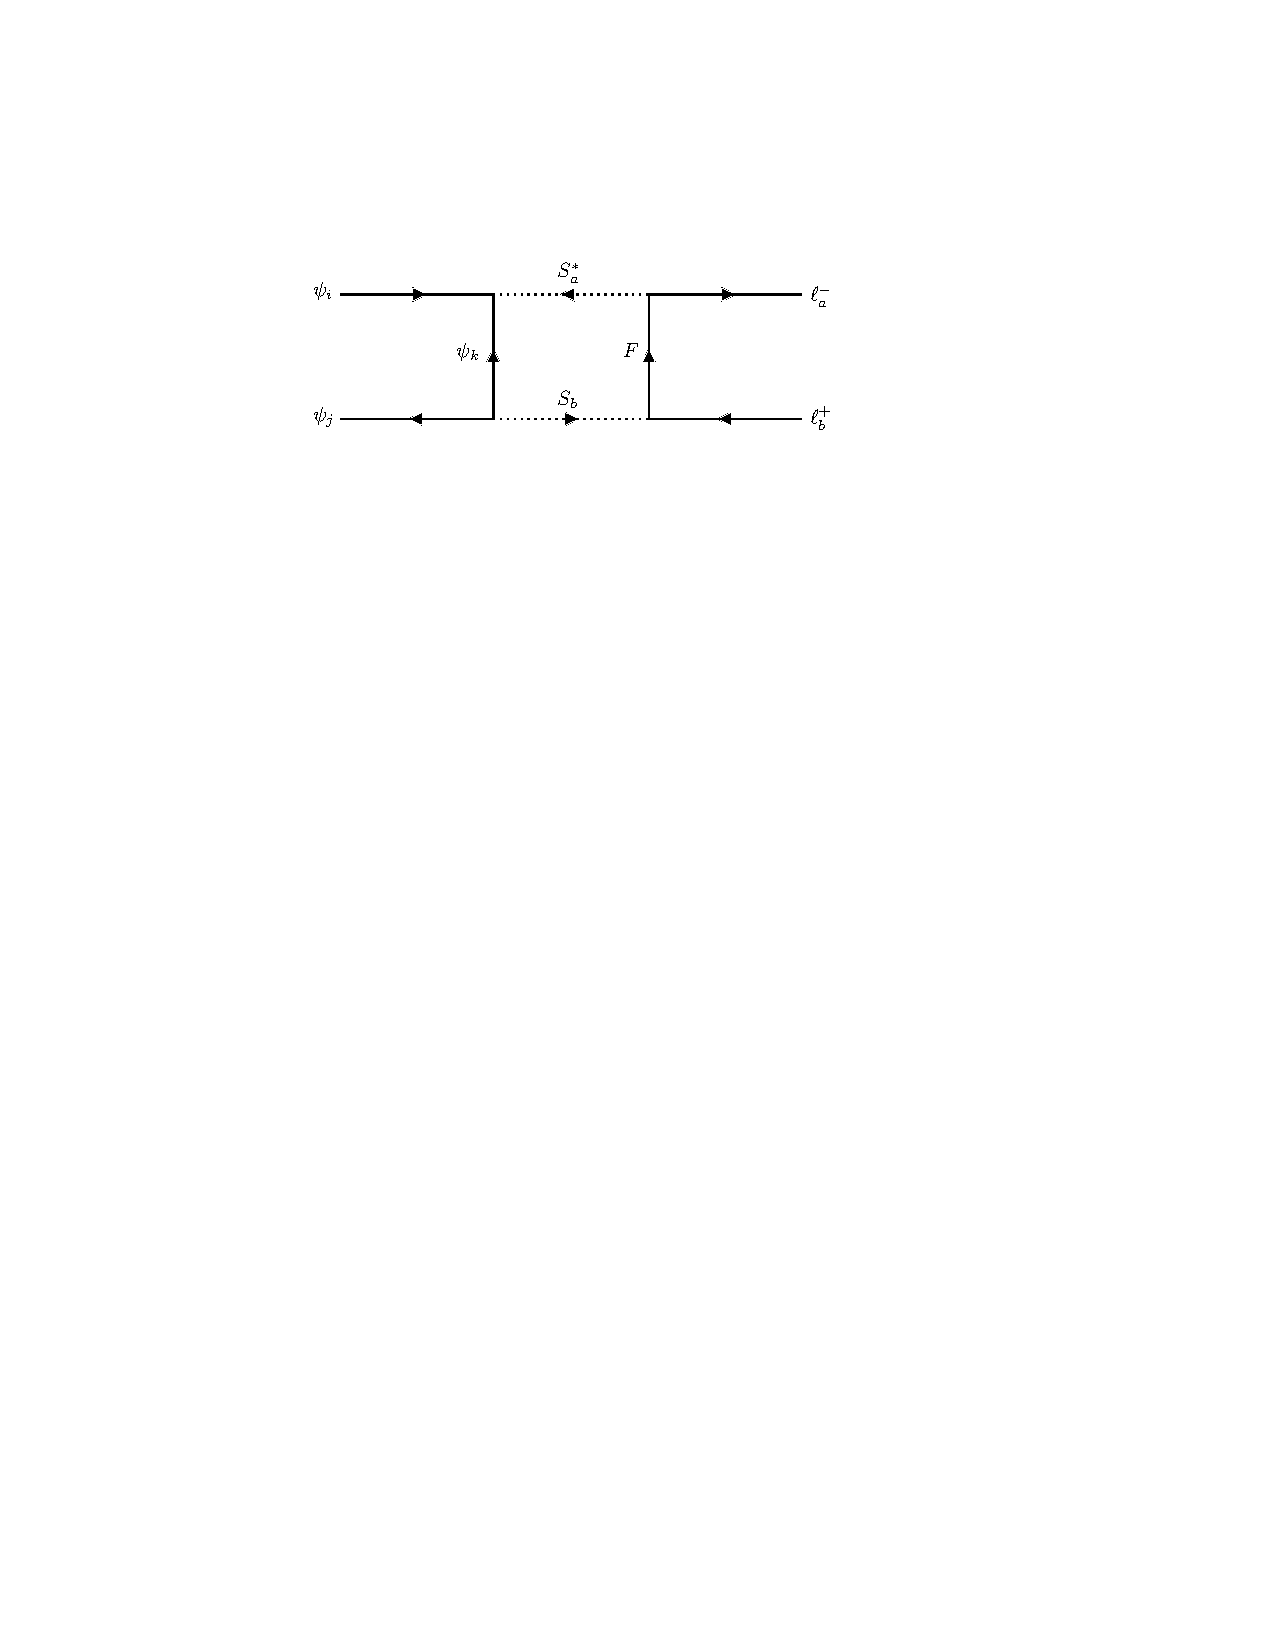
\includegraphics[width=0.8\linewidth]{figures/appendixA/dark_pion_matching_diagram.pdf}
    \caption[UV matching diagram]{A diagram in the UV theory which can be matched onto $\Pi\rightarrow \ell_a^- \ell_b^+$ in the low-energy EFT. Note that the arrow on the internal $\psi_k$ line is reversed, due to the presence of a charge conjugation operator in the $S$ interaction in \ref{eq:UV_lag}.}
    \label{fig:matching_diagram}
\end{figure}
Using the Feynman rules for the Lagrangian (\ref{eq:UV_lag}), the amplitude can be expressed in the form
\begin{align}
    i{\cal M} &= \lambda_a'\lambda_b'^* N_c \bar{v}(p_j)\gamma^5 \left[G^{ij-}_{ab} \gamma_\nu {\cal I}_1^{\mu\nu} + G^{ij+}_{ab}{\cal I}_2^{\mu} \right]u(p_i)\bar{u}(k_a)\gamma_\mu P_L v(k_b)
\end{align}
where $N_c$ is a dark color factor, $p_i$ and $p_j$ are the momenta of the dark quarks $\psi_i$ and $\psi_j$, $k_a$ and $k_b$ are the momenta of the leptons $\ell_a$ and $\ell_b$, $G_{ab}^{ij\pm} = g_{aS}^{ij}g_{bPS}^{ij*} \pm g_{aPS}^{ij}g_{bS}^{ij*}$, and ${\cal I}_1$ and ${\cal I}_2$ are integral expressions given by
\begin{align}
    {\cal I}_1^{\mu\nu} &= \int{\frac{d^4q}{(2\pi)^4}\frac{q^\nu}{q^2 - m^2}}\frac{1}{(p_i+q)^2 - M_S^2}\frac{1}{(p_j - q)^2 - M_S^2}\frac{p_i^\mu+q^\mu - k_a^\mu}{(p_i+q-k_a)^2 - M_F^2},\\
    {\cal I}_2^\mu &= \int{\frac{d^4q}{(2\pi)^4}\frac{m_k}{q^2 - m^2}}\frac{1}{(p_i+q)^2 - M_S^2}\frac{1}{(p_j - q)^2 - M_S^2}\frac{p_i^\mu+q^\mu - k_a^\mu}{(p_i+q-k_a)^2 - M_F^2}.
\end{align}
These integrals have solutions (to lowest order in $m/M_F, m/M_S$), 
\begin{align}
    & I_{1}^{\mu\nu} = \frac{ig^{\mu\nu}}{16\pi^2 M_S^2}g_1(M_F^2/M_S^2),
    & I_{2}^{\mu} = \frac{i}{16\pi^2 M_S^2}\frac{m(p_i^\mu - k_a^\mu)}{M_S^2}g_2(M_F^2/M_S^2), &
\end{align}
where
\begin{align}
    & g_1(x) = \frac{1-x+x\log{x}}{(1-x)^2},
     & g_2(x) = \frac{1-x+\log{x}}{(1-x)^2}. &
\end{align}
Taking $M_F \approx M_S$, we note that $\lim_{x\rightarrow 1}g_1(x) = -\lim_{x\rightarrow 1}g_2(x) = 1/2$. In addition, $I_2 \ll I_1$ due to a suppression of $m_k/M_S$ (and a potential additional suppression by $(p_i^\mu - k_a^\mu)/M_S$ as well depending on the energy scale of the interaction). Finally, we note that the color factor is $N_C = \epsilon_{\alpha\beta\gamma}\delta_{\delta}^{\gamma}\epsilon^{\rho\sigma\tau}\delta_{\tau}^{\beta}=\epsilon_{\alpha\beta\gamma}\epsilon^{\gamma\sigma\beta} = 2\delta_\alpha^\sigma$. Hence, the amplitude at low energy scales ($\ll M_S$) can be written
\begin{align}
    i{\cal M} &\approx \frac{\lambda_a'\lambda_b'^* G_{ab}^{ij-}}{16\pi^2 M_S^2}[\bar{v}(p_j)\gamma^5 \gamma^\mu u(p_i)][ \bar{u}(k_a) \gamma_\mu P_L v(k_b)],
\end{align}
corresponding to an effective interaction 
\begin{align}
    {\cal L}_{\psi\psi\ell\ell} &= \sum_{a,b}\frac{\lambda_a'\lambda_b'^*}{16\pi^2 M_S^2} \sum_{i,j}\left[iG_{ab}^{ij-}\bar{\psi}_j \gamma^\mu \gamma^5 \psi_i\right]_{{\Bbb Z}_2 = +} \bar{\ell}_a \gamma_\mu P_L \ell_b. \label{eq:dark_quark_eff_int}
\end{align}
where we have placed the factor of $i$ adjacent to $G_{ab}^{x-}$ to emphasize that $G_{ab}^{x-}$ is {\it anti-Hermitian} in the lepton indices $a$,$b$.
\subsection{Dark Pion Matching}
Treating the dark quarks $\psi_i$ as a global $SU(3)$ triplet, the interaction Lagrangian (\ref{eq:dark_quark_eff_int}) can be written in the form 
\begin{align}
    {\cal L}_{\psi\psi\ell\ell} &= \sum_{a,b}\frac{\lambda_a'\lambda_b'^*}{16\pi^2 M_S^2} \sum_{i,j}{
    i\bar{\boldsymbol \psi}{\bf G}_{ab}^{-}\gamma^\mu \gamma^5{\boldsymbol{\psi}} }\bar{\ell}_a \gamma_\mu P_L \ell_b.
\end{align}
where
\begin{align}
   \setlength{\arraycolsep}{0.1cm}\renewcommand{\arraystretch}{0.6}  {\boldsymbol \psi} \equiv \begin{pmatrix}\psi_1 \\ \psi_2 \\ \psi_3 \end{pmatrix}\ \ \ {\rm and} \ \ \ {\bf G}_{ab}^{-} \equiv \begin{pmatrix}G^{11-}_{ab} & G^{12-}_{ab} & 0 \\ G^{21-}_{ab} & G^{22-}_{ab} & 0 \\ 0 & 0 & G^{33-}_{ab}\end{pmatrix}
\end{align}
and $G_{ab}^{i3-} = G_{ab}^{3i-} = 0$ for $i = 1, 2$ to enforce the ${\Bbb Z}_2$ symmetry. We wish to match onto the ${\Bbb Z}_2$-even dark pions $\Pi_x \in \{\pi_D, \pi_D', \bar{\pi}_D', \eta_D\}$. To do so, we note that the overlap between the axial current operator and the pion wavefunction is given by
\begin{align}
    \langle 0|\bar{\psi}_i \gamma^\mu\gamma^5 \lambda^x_{ij}\psi_j|\Pi_y(p)\rangle &= ip^\mu F_{\Pi_y}\delta^{x}_{y}.
\end{align}
Hence, in order to find the contribution of the dark quark effective interaction Lagrangian to the pion interactions, we must decompose the interaction matrix ${\bf G}_{ab}^-$ into the identity and Gell-Mann matrices ${\bf G}_{ab}^- = G_{ab}^{0-}{\bf 1} + \sum_{z}G_{ab}^{x-}\lambda^{x}$, which is always possible for a $3\times 3$ complex Hermitian matrix. We can invert this equation using the property $\sum_{i,j} \lambda_{ij}^x\lambda_{ij}^y = 2\delta^{xy}$ ,so $G_{ab}^{x-} = \frac{1}{2}\sum_{i,j}\lambda_{ij}^x G_{ab}^{ij,-}$. Explicitly,
\begin{align}
    G_{ab}^{\pi-} &= \frac{1}{2}(G_{ab}^{11-} -G_{ab}^{22-} )\\
    G_{ab}^{\bar{\pi}'-} &= \frac{1}{\sqrt{2}}G_{ab}^{12-},\\
    G_{ab}^{\pi'-} &= \frac{1}{\sqrt{2}}G_{ab}^{21-},\\
    G_{ab}^{\eta -} &= \frac{1}{2\sqrt{3}}(G_{ab}^{11-} + G_{ab}^{22-} - 2 G_{ab}^{33-}).
\end{align}
Then, the effective lepton-pion interaction strength is given by
\begin{align}
    \frac{C_{ab}^x}{\Lambda} &= \frac{\lambda_a'\lambda_b'^*}{16\pi^2}\frac{F_{\Pi_x}}{M_S}\frac{iG_{ab}^{x-}}{M_S}
\end{align}
In terms of the original parameters of the UV Lagrangian
\begin{equation}
\frac{C_{ab}^x}{\Lambda} = \frac{\lambda_a^\prime\lambda_b^{\prime*}}{32\pi^2M_S}\sum_{i,j}i\left[g_{aS}^{ij}g_{bPS}^{ij*} - g_{aPS}^{ij}g_{bS}^{ij*}\right]\frac{F_{\Pi_x}}{M_S}\lambda_{ij}^x.
\end{equation}
In the event that the dark pions $\Pi^-$ are nearly degenerate, we can approximately match this onto the ALP EFT (\ref{eq:ALP_EFT}) parameter $C_{\ell\ell'}$. Roughly,
\begin{align}
    \frac{C_{\ell\ell'}}{\Lambda} \sim \frac{\lambda'^2 g^2}{32\pi^2 M_S}\frac{F_\Pi}{M_S}.
\end{align}
Adopting the numerical values for the benchmark UV model in \cite{Davoudiasl:2017zws} of $\lambda' \approx 0.1$,  $g \approx 0.3$, $F_\Pi \sim 80$ GeV, and $M_S \sim 1$ TeV we find the numerical value
%
\begin{equation}
\frac{|C_{\ell \ell'}|}{\Lambda} \approx 2 \times 10^{-7}\ {\rm TeV}^{-1}.
\end{equation}
So while the Higgs coupling $C_{ah}'/\Lambda^2$ from this model is quite large, the lepton coupling $C_{\ell\ell'}/\Lambda$ is substantially smaller, too weak to be probed at current experiments. However, given the flavor-violating nature of the interaction, such a coupling may be probed at experiments in the near future, as discussed in the text.